\documentclass[12pt, letter]{exam}
\usepackage[utf8]{inputenc}
\usepackage[T1]{fontenc}
\usepackage[spanish]{babel}
\usepackage[autostyle,spanish=mexican]{csquotes}
\usepackage{amsmath}
\usepackage{amsthm}
\usepackage{physics}
\usepackage{tikz}
\usepackage{float}
\usepackage{siunitx}
\usepackage{multicol}
\usepackage{enumitem}
\usepackage[left=2.00cm, right=2.00cm, top=2.00cm, 
     bottom=2.00cm]{geometry}
\usepackage{pdfpages}

% \renewcommand{\questionlabel}{\thequestion}
\decimalpoint

\setlength{\belowdisplayskip}{-0.5pt}

\usepackage{tasks}
\settasks{
    label=\Alph*), 
    label-align=left,
    item-indent={20pt}, 
    column-sep={4pt},
    label-width={16pt},
}

\sisetup{per-mode=symbol}
\footer{}{\thepage}{}

\begin{document}

\includepdf[pages=-]{Caratula_Examen_Parcial_04_PU_Fisica_3_03_Grupo_43.pdf}

\setcounter{page}{3}

\begin{center}
\textbf{Cada ejercicio vale 1 punto, incluidos los ejercicios de ejecución.}
\end{center}

\begin{questions}
    \section{(7 puntos) Movimiento circular.}

    \question Identifica de la siguiente figura los elementos del círculo.
    \begin{figure}[H]
        \centering
        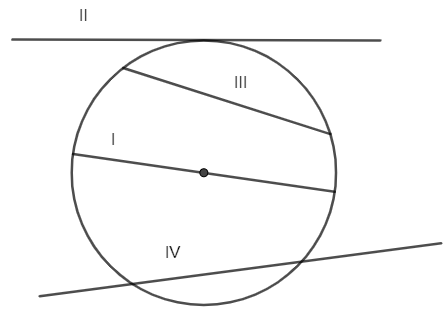
\includegraphics[scale=1]{Elementos_Circulo_02.png}
    \end{figure}
    \begin{multicols}{2}
    \begin{parts}
        \part Radio
        \part Cuerda
        \part Tangente
        \part Secante
        \part Centro
        \part Diámetro
    \end{parts}
    \end{multicols}
    
    \vspace*{0.25cm}
    Respuestas:
    \begin{multicols}{2}
    \begin{tasks}
        \task f-I, c-II, b-III, d-IV
        \task e-I, a-II, d-III, b-IV
        \task f-I, d-II, c-III, a-IV
        \task a-I, b-II, c-III, d-IV
    \end{tasks}
    \end{multicols}
    \question En el movimiento circular las unidades de frecuencia son: \rule{2cm}{0.1mm}
    \begin{tasks}(4)
        \task $\displaystyle \unit[per-mode=fraction]{\radian\per\second}$
        \task $\displaystyle \unit[per-mode=fraction]{\meter\per\second}$
        \task $\displaystyle \unit[per-mode=fraction]{\radian\per\square\second}$
        \task $\dfrac{1}{\unit{\second}}$
    \end{tasks}
    \question Considerando el radio (r), el radián se define como el ángulo central al que corresponde un arco de longitud igual: \rule{2cm}{0.1mm}.
    \begin{tasks}(4)
        \task $\dfrac{\pi}{2} \, r$
        \task $r$
        \task $\pi \, r$
        \task $2 \, r$
    \end{tasks}
    \question ¿Cuál es la trayectoria de la velocidad lineal de un objeto que describe un movimiento circular?
    \begin{tasks}(4)
        \task Una cuerda.
        \task Una secante.
        \task Una tangente.
        \task Un radio.
    \end{tasks}
    \question \label{Ejercicio_01} \textbf{Ejercicio de ejecución: } Convierte $4.5 \, \pi$ radianes a grados.
    \begin{tasks}(4)
        \task \ang{720}
        \task \ang{810}
        \task \ang{900}
        \task \ang{990}
    \end{tasks}
    \question \label{Ejercicio_02} \textbf{Ejercicio de ejecución: } Las aspas de una licuadora giran a razón de \num{6500} rpm. Cuando el motor se apaga durante la operación, las aspas frenan hasta llegar al reposo en \SI{4.0}{\second}. ¿Cuál es la aceleración angular conforme frenan las aspas?
    \begin{tasks}(4)
        \task $\displaystyle - \SI{170.16}{\radian\per\square\second}$
        \task $\displaystyle - \SI{190.44}{\radian\per\square\second}$
        \task $\displaystyle - \SI{242.93}{\radian\per\square\second}$
        \task $\displaystyle - \SI{258.62}{\radian\per\square\second}$
    \end{tasks}
    \question \label{Ejercicio_03} \textbf{Ejercicio de ejecución: } Una rueda de molino de \SI{0.35}{\meter} de diámetro gira a \num{2500} rpm. ¿Cuál es la aceleración centrípeta de un punto localizado en el borde de la rueda de molino?
    \begin{tasks}(4)
        \task $\displaystyle \SI[per-mode=fraction]{978.89}{\meter\per\square\second}$
        \task $\displaystyle \SI[per-mode=fraction]{10500.19}{\meter\per\square\second}$
        \task $\displaystyle \SI[per-mode=fraction]{11564.24}{\meter\per\square\second}$
        \task $\displaystyle \SI[per-mode=fraction]{11990.47}{\meter\per\square\second}$
    \end{tasks}
    
    \section{(4 puntos) Piezoelectricidad.}

    \question Son materiales que presentan el efecto piezoeléctrico:
    \begin{multicols}{2}
    \begin{tasks}
        \task Cristales, Líquidos, Cerámicos.
        \task Cristales, Materia orgánica, Gases.
        \task Cristales, Cerámicos, Polímeros.
        \task Plásticos, Cerámicos, Polímeros.
    \end{tasks}
\end{multicols}
    \question Una de las propiedades de los cerámicos es la \rule{2cm}{0.1mm}

    \vspace{0.5cm}
    \begin{multicols}{2}
        \begin{tasks}
            \task Resistencia a la temperatura
            \task Conductividad eléctrica
            \task Alta Densidad
            \task Alta Ductibilidad
        \end{tasks}
    \end{multicols}
    \question La piezoelectricidad es un fenómeno físico en el cual ciertos materiales tienen la capacidad de generar una \rule{2cm}{0.1mm} eléctrica.
    \begin{tasks}(4)
        \task Resistencia
        \task Carga
        \task Conductividad
        \task Permeabilidad
    \end{tasks}
    \question En la transformación de energía mecánica a eléctrica en un material piezoeléctrico, al deformarse la estructura del material se genera: \rule{2cm}{0.1mm}
    \begin{tasks}(4)
        \task Resistencia
        \task Potencia
        \task Fuerza
        \task Voltaje
    \end{tasks}

    \section{(4 puntos) Superconductividad.}

    \question De la relación entre resistividad y conductividad sabemos que: a \rule{2cm}{0.1mm} sea la su conductividad de un material, \rule{2cm}{0.1mm} será resistencia eléctrica.
    \begin{tasks}(4)
        \task Mayor - Mayor
        \task Mayor - Menor
        \task Igual - Igual
        \task Menor - Menor
    \end{tasks}
    \question El valor de temperatura en el que se presenta el estado superconductor en un material, se le conoce como \rule{2cm}{0.1mm}
    \begin{multicols}{2}
    \begin{tasks}
        \task Temperatura mínima.
        \task Temperatura máxima.
        \task Temperatura crítica.
        \task Temperatura estándar.
    \end{tasks}
    \end{multicols}
    \question Un material superconductor se caracteriza por que su resistencia interna \rule{2cm}{0.1mm}
    \begin{tasks}(4)
        \task Se incrementa.
        \task Se hace negativa.
        \task No cambia.
        \task Es cero.
    \end{tasks}
    \question Una de las características de un material superconductor es que repele un campo magnético externo, lo que se conoce como efecto: \rule{2cm}{0.1mm}
    \begin{tasks}(4)
        \task Tesla
        \task Meissner
        \task Faraday
        \task Cherenkov
    \end{tasks}

    \section{(5 puntos) Sustentabilidad y contaminación.}

    \question Cuando nos referimos a la capacidad de satisfacer las necesidades actuales de la sociedad sin comprometer la capacidad de las futuras generaciones para satisfacer sus propias necesidades, hablamos de: \rule{2cm}{0.1mm}
    \begin{tasks}(4)
        \task Sostenibilidad
        \task Sustentabilidad
        \task Economía
        \task Crecimiento
    \end{tasks}
    \question La Asamblea General de las Naciones Unidas en 2009 estableció el Día Internacional de la Madre Tierra, que se celebra el \rule{2cm}{0.1mm} de cada año como un recordatorio de la importancia de cuidar y proteger nuestro planeta.
    \begin{tasks}(4)
        \task 1 de mayo
        \task 9 de septiembre
        \task 22 de abril
        \task 4 de enero
    \end{tasks}
    \question Este fenómeno ocurre cuando ciertos gases en la atmósfera terrestre retienen el calor emitido por la Tierra y lo reenvían de vuelta a la superficie, lo que produce un aumento de la temperatura global: \rule{2cm}{0.1mm}
    \begin{tasks}(4)
        \task Efecto invernadero
        \task Inversión térmica
        \task Cambio climático
        \task Contaminación del aire
    \end{tasks}
    \question La inversión térmica es un fenómeno que se presenta cuando la temperatura del aire \rule{2cm}{0.1mm} conforme subimos en altura.
    \begin{tasks}(4)
        \task Aumenta
        \task No cambia
        \task Disminuye
        \task Se anula
    \end{tasks}
    \question Las partículas PM2.5 son aquellas partículas sólidas o líquidas de diferente composición y tamaño que se encuentran dispersas en la atmósfera y que tienen un diámetro \rule{2cm}{0.1mm}
    \begin{tasks}(4)
        \task Mayor que \SI{2.5}{\micro\meter}
        \task Menor que \SI{2.5}{\micro\meter}
        \task Igual a \SI{0.25}{\micro\meter}
        \task Igual a \SI{0.025}{\micro\meter}
    \end{tasks}

\end{questions}


\end{document}